% ----------------------------------------------------------------
% Article Class (This is a LaTeX2e document)  ********************
% ----------------------------------------------------------------
\documentclass[11pt]{article}
\usepackage[english]{babel}
\usepackage{amsmath,amsthm, amssymb}
\usepackage{amsfonts}
\usepackage{multirow}
\usepackage{threeparttable}

%Candelaria's favorite packages
\usepackage{setspace}	% Set the spacing for the document
\usepackage{xtab}		% Use for tables
\usepackage{comment}	% Use for block comments
\usepackage{rotating}	% Helpful for rotating figures
\usepackage{lscape}	% Change a page into landscape
\usepackage{hyperref}
\hypersetup{colorlinks=false,pdfborder={0 0 0},breaklinks=true}
\usepackage{graphicx}	% Load a graphic image
%\usepackage{url}		% Use for formatting URLS (nice for NatBib also)
\usepackage{booktabs}  	% Use for nice tables/ Works well with ESTOUT
\usepackage{longtable} 	% Used to break long tables over multiple pages
\usepackage{caption}
\usepackage{subcaption} 	% Used to create SubFloats
\usepackage{listings} 	% Use to enter code blocks, like a fancy verbatim

% ADD COLOR:
\usepackage{color}
\usepackage[usenames, dvipsnames, svgnames, table]{xcolor}

% Packages for the bibliography
\usepackage[longnamesfirst]{natbib}
%\usepackage{natbib}

% Set Page Margins
%\usepackage{fullpage}
\addtolength{\oddsidemargin}{-.875in}
\addtolength{\evensidemargin}{-.875in}
\addtolength{\textwidth}{1.75in}
\addtolength{\topmargin}{-.875in}
\addtolength{\textheight}{1.75in}

% Set line and table spacing
\renewcommand{\baselinestretch}{1.0}
\renewcommand{\arraystretch}{1.1}
\setlength\abovedisplayskip{0pt}
\setlength\belowdisplayskip{0pt}

% Redefine the cite command
\renewcommand\cite{\citet}

%\setlength{\parindent}{0in}

%\setlength{\leftmargin}{0pt} \setlength{\parskip}{1.1ex} \setlength{\parindent}{1em} \setlength{\itemsep}{0pt} \setlength{\footnotesep}{10pt}
%\renewcommand{\footnoterule}{\rule{3in}{.3pt}\vspace{-.3pt}}

% THEOREMS -------------------------------------------------------
\newtheorem{thm}{Theorem}[section]
\newtheorem{cor}[thm]{Corollary}
\newtheorem{lem}[thm]{Lemma}
\newtheorem{prop}[thm]{Proposition}
\theoremstyle{definition}
\newtheorem{defn}[thm]{Definition}
\theoremstyle{remark}
\newtheorem{rem}[thm]{Remark}
%\numberwithin{equation}{section} %Number equations within section
% ----------------------------------------------------------------

%%%%%%TYPESET LINEAR EQUATIONS
\usepackage{environ}

\makeatletter

\newcommand{\LinearSystems@SetupLets}{%
  \let\col=&%
  \let\+=+%
  \let\-=-%
  \let\===%
}
\newcommand{\LinearSystems@SetupCatcodes}{%
  \catcode`\&=\active
  \catcode`\+=\active
  \catcode`\-=\active
  \catcode`\==\active
}
\newcommand{\LinearSystems@Setup}{}
\begingroup
  \LinearSystems@SetupCatcodes
  \gdef\LinearSystems@Setup{%
    \LinearSystems@SetupLets
    \LinearSystems@SetupCatcodes
    \newcommand&[1][0pt]{\col\hspace{##1}\col}%
    \def+{\col\+{}{}\col}%
    \def-{\col\-{}{}\col}%
    \def={\col\={}{}\col}%
  }
\endgroup

\NewEnviron{LinearSystems}[1]{\begin{alignat*}{#1}\BODY\end{alignat*}}
\let\LinearSystems@OriginalBegin\LinearSystems
\def\LinearSystems{\LinearSystems@Setup\LinearSystems@OriginalBegin}

\makeatother
%%%%%%%%%%%%%%%%%%%%%%%%





% AUTHOR INFO


\title{Lecture 1: Algebra and Precalculus \\ September 4, 2018}%

% ----------------------------------------------------------------

%%%%%%
% SHORT CITES
%%%%%%
\shortcites{ColEtAl1966}


\begin{document}

\begin{center}
{\huge Pre-Calculus Lecture Notes\footnote{Contributor(s): Chris Candelaria, Erin Fahle, Betsy Williams, and Klint Kanopka. If you find errors, please let Klint know so that he may correct them. Thanks!}}\\[5pt]
{\Large Stanford GSE Math Camp \\[5pt]
Do Not Distribute Outside GSE}
\end{center}

\section{Software Packages of Interest}
    \subsection{Document Processing}
    	\begin{itemize}
        	\item \textbf{Microsoft Word - } Basically everyone uses this.  Some advisors are crazy about ``track changes'' on working documents.  You'll need a copy of this to make sure things are formatted in a non-awful manner. 
            \item \LaTeX - This document was formatted using \LaTeX.  
            Pros: 
            \begin{itemize}
                \item Looks great. 
                \item Handles equations really well.  
                \item Flexible.
                \item Free.  
            \end{itemize}
            Cons: 
            \begin{itemize}
                \item Can be extremely frustrating.
                \item Not straightforward to learn.
                \item Many people can't deal with .tex files and .pdfs can be hard to collaborate on.
                \item Some journals prefer .docx submissions.
            \end{itemize}
            If you want to try it out, \LaTeX is easily accessible from native clients (TexPad, TexShop, TexWorks, etc) or compiled from a text editor of your choice (Sublime Text, Atom, VIM).  Also really easy to use online (Overleaf). Overleaf has also been steadily improving their collaboration features.
            \item \textbf{Markdown - } The README on the github repo was written in markdown. It generally has fewer options than \LaTeX, but is easier to deal with. It's also built into RSTudio (if you're an R user).
        \end{itemize}
        
   	\subsection{Citation Managers}
    	\begin{itemize}
        	\item \textbf{Mendeley - } Citation manager.  I use this one because it has the least-awful Linux client. Stanfod once had an instiutional license, but has since cancelled it.
            \item More than I care to mention exist (Zotero and EndNote are the other two I'm aware of).  A good comparison is available here:  https://guides.library.utoronto.ca/c.php?g=250610\&p=1671260 
        \end{itemize}

    \subsection{Quantitative Software}
    	\begin{itemize}
        	\item \textbf{Excel - } Spreadsheet program on almost everyone's computer.  Pros: You probably already know how to use it.  Lots of buttons, so it's pretty easy to figure out.  Good for quick tasks.  Cons: Slow with large data sets.  Shameful to use for ``real'' work, because work done in Excel (or any other spreadsheet) is not easily reproducable. 
            \item \textbf{SPSS - } Statistical Package for Social Science (I think?).  Popular amongst faculty trained in Psychology.  Pros: Lots of buttons, so it works like a super-powerful Excel.  Has support for scripting and syntax, so can be used conduct reproducable research.  Cons: Not popular among faculty not trained in Psychology.
            \item \textbf{SAS - } Statistical Analysis Software.  Pros: Good for large data sets and data cleaning.  Cons: I don't know of anyone in the GSE who uses it, so support will be thin if you're picking it up for the first time.
        	\item \textbf{Stata - } Statistical software popular among the Econ crowd.  Pros: Every class in the 400 and 430 sequence in the GSE is taught in Stata.  There is no easier way to work with large panel data sets. Commands are easy to learn and do files help you automate or reproduce tasks.  Your advisor probably uses Stata. Your advisor will probably buy you Stata.  Cons:  Not free.  Making attractive plots can be annoying, but not impossible.
            \item \textbf{R - } A (quirky) programming language that gets pitched as statistical software.  Pros: Free.  Packages exist to do pretty much whatever you'd like.  Popular in the data science community.  Cons:  Very steep learning curve, especially if you have no prior programming experience. Really weird syntax.  All arrays are 1-indexed, so if you have prior programming experience, this will cause you headaches to no end. 
            \item \textbf{Python - } Interpreted programming language.  Pros: Free. Fast. Popular in the data science community and can be used for a whole bunch of non-statistical applications.  Cons: Steep learning curve.  Some of the stats plugins are even less friendly here than in R.
        \end{itemize}
        
    \subsection{VPN}
		\begin{itemize}
        	\item \textbf{Cisco VPN - } Worth the effort to set up if you live off-campus or travel often.  Allows access to journals, data, library materials, and anything else that requires you be on the Stanford network from anywhere in the world. Instructions available at:  uit.stanford.edu/service/vpn 
        \end{itemize}
\section{Review of Algebra and Notation}


\subsection{Order of Operations}
\begin{itemize}
\item \textbf{Basic Algebraic Symbols:}
\begin{itemize}
\item Addition ($+$), subtraction ($-$), multiplication ($\times$ or $*$), division ($\div $ or $/ $)
\item Sum ($\sum $, $\sum\limits_{a \in A} $, or  $\sum\limits_{i=1}^N$), product ($\prod $,  $\prod\limits_{a\in A} $,  or $\prod \limits_{i=1}^N$)

\end{itemize}
\item \textbf{PEMDAS:}
\begin{itemize}
\item \textbf{P}lease \textbf{E}xcuse \textbf{M}y \textbf{D}ear \textbf{A}unt \textbf{S}ally 
\item \textbf{P}arentheses \textbf{E}xponents \textbf{M}ultiplication \textbf{D}ivision \textbf{A}ddition \textbf{S}ubtraction
\end{itemize}
\item \textbf{Exercises:} 
\begin{enumerate}
\item Evaluate $\sum\limits_{x=1}^5 x$
\item Solve for x: $50 = 5(x+2) + 5$
\item Evaluate: $\displaystyle \prod_{x=1}^3 (x-1)$
\end{enumerate}
 \end{itemize}
\subsection{Working with Units}
\begin{itemize}

\item Remember that units multiply and divide, too!
\begin{itemize}
\item Driving at 60 miles/hour for 2 hours takes you 120 miles, because  $\dfrac{hours}{hours}$ cancels out.
$$ 2~hours \times 60~miles/hour = 120~miles$$
\item A rectangular neighborhood that is 2 km by 3 km has an area of 6 square km.\\ 
$$2~km \times 3~km = 6~km^2$$
\item A proportion has no units. A cake recipe that uses 2 1/2 cups sugar and 3 1/2 cups flour has a ratio of 5 parts sugar to 7 parts flour, whether you double the recipe or measure it again in metric units. 
$$2.5~cups:3.5~cups = 5:7$$
\end{itemize}
\end{itemize}


\subsection{Exponents}
\begin{itemize} 
\item \textbf {Rules of Exponents} If $a$ and $b$ are positive numbers, $n$ is a positive integer, and $x$ and $y$ are any real numbers, then:
\begin{enumerate}
\item $a^n = \underbrace{a \times a \times a \times \cdots \times a}_n$
\item $a^0 = 1$
\item $a^{-1} = \displaystyle \frac{1}{a}$
\item $a^{x+y}=a^x a^y$
\item $a^{x-y}= \displaystyle \frac{a^x}{a^y}$
\item $(a^x)^y = a^{xy}$
\item $(ab)^x = a^x b^x$
\item $\displaystyle \left( \frac{a}{b} \right)^x = \frac{a^x}{b^x}$
\item $a^{\frac{1}{2}} = \sqrt{a}$
\item $\sqrt[x]{a} = a^{\frac{1}{x}}$
\end{enumerate}
\item \textbf{Exercises:}
\begin{enumerate}
\item Evaluate: $(5 \times 4)^2$
\item Evaluate: $((1+3)^3)^2 \times 2 + 5$
\end{enumerate}
\end{itemize}

\subsection{The Coordinate Plane:} There are four \textbf{quadrants} on a coordinate plane (labeled below). The horizontal axis is known as the x-axis and the vertical axis is known as the y-axis. Coordinates of the form (x,y) are plotted on this plane. \\
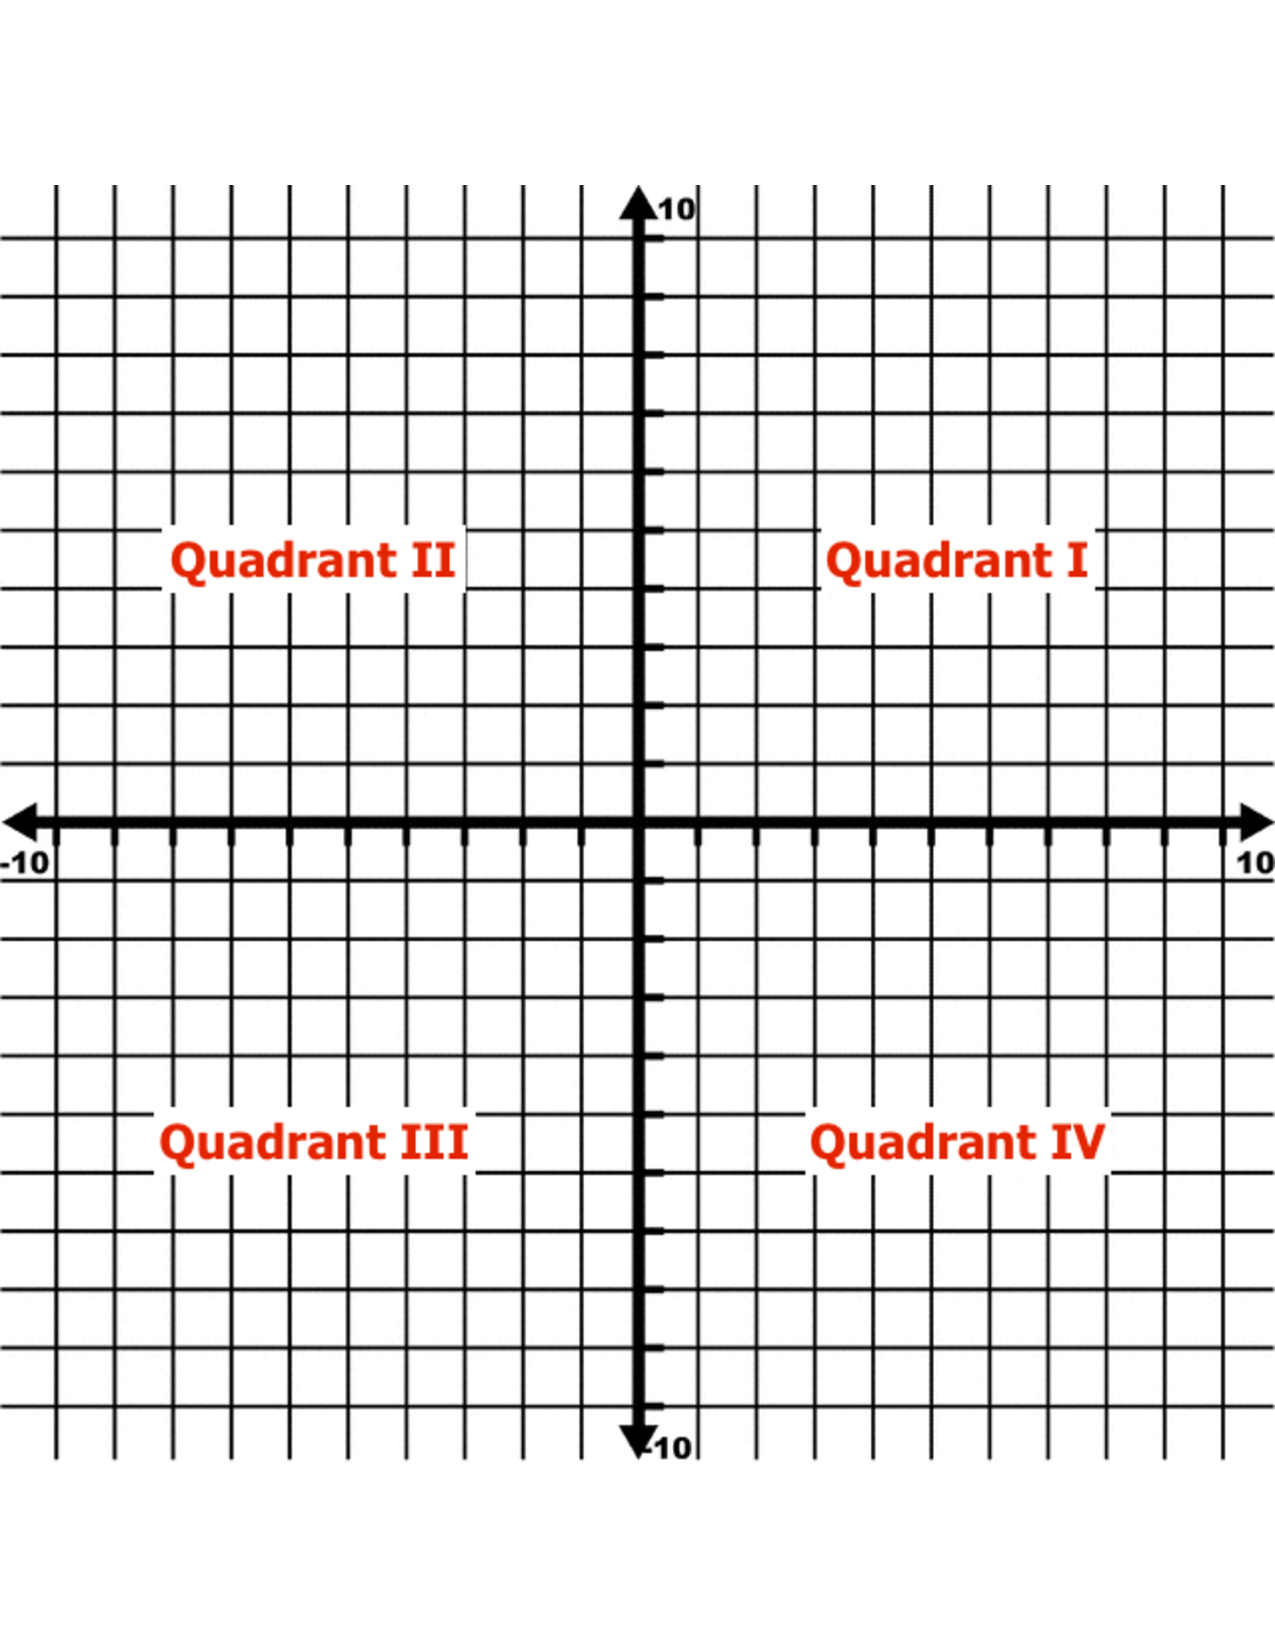
\includegraphics[scale=0.3, trim=-450 100 0 50]{img/coordplan_quadlab.pdf}
\begin{itemize}
\item Point on the coordinate plane are represented as couples of numbers, e.g. $P_1 = (x_1, y_1)$
\item \textbf{Distance Formula:} The distance between two points $P_1 = (x_1, y_1)$ and $P_2 = (x_2, y_2) $ in the x-y plane is given by:
\begin{equation*}
|P_1P_2| = \sqrt[]{(x_2-x_1)^2+(y_2-y_1)^2}
\end{equation*}
\item \textbf{Exercises:}
\begin{enumerate}
\item Can you plot the points (1,2) and (3,-2) on the coordinate plane and find the distance between them?
\item Demonstrate that the Pythagorean Theorem and the distance formula are equivalent. Remember, the PT says:  in a right triangle, where a and b are the lengths of sides next to the right angle, and c is the length of the hypotenuse, the lengths have the relationship
\end{enumerate}
\begin{equation*}
a^2 + b^2 = c^2
\end{equation*}
\end{itemize}

\subsection{Lines:}

\begin{itemize}

\item \textbf{Slope of a Line}: The slope of a line passing through the points $P_1 = (x_1, y_1)$ and $P_2 = (x_2, y_2) $ is 
\begin{equation*}
m=\displaystyle \frac{\Delta y}{\Delta x}  = \displaystyle \frac{y_2 - y_1}{ x_2 - x_2} = \displaystyle \frac{rise}{run}
\end{equation*}
\item\textbf{Equation of a Line:}
\begin{enumerate}
\item \textbf{Point-Slope Form:} Given a point, $P_1 = (x_1, y_1)$, and a slope, m, you can plot the line:
\begin{equation*}
y-y_1 = m(x - x_1)
\end{equation*}
\item \textbf{Slope-Intercept Form:} Given a slope, m, and the y-intercept, (0,b), you can plot the line:
\begin{equation*}
y = mx + b
\end{equation*}

\item \textbf{Terminology:}
\begin{enumerate}
\item \textbf{Parallel:} Two lines are parallel if and only if they have the same slope.
\item \textbf{Perpendicular:} Two lines are perpendicular if and only if their slopes, $m_1$ and $m_2$, are negative reciprocals, i.e. $m_1m_2 = -1$, $m_1 =\frac{-1}{m_2}$
\end{enumerate}
\end{enumerate}

\item \textbf{Linear Regression:}
\begin{itemize}
    \item Linear relationships form the basis of much quantitative education research. For a dependent variable, $Y$, with a single independent variable, $X$, we can write:
    $$ Y = \beta_0 + \beta_1 X$$
    \item We interpret this as ``A one unit change in $X$ is associated with a $\beta_1$ unit change in $Y$.''
    \item This works for multiple independent variables, too!
    \item To learn more about this, take EDUC400B, EDUC430A, EDUC430B, or equivalent courses in other departments.
\end{itemize}

\item \textbf{Exercises:}
\begin{enumerate}
\item Plot the line through the points $(1,2)$ and $(4,3)$. 
\begin{enumerate}
\item What is the slope? 
\item What is the intercept?
\end{enumerate}
\item A researcher runs a regression of SAT Math score on age and finds the relationship: $$SAT_{Math,i} = 30 \times AGE_i$$.
\begin{enumerate}
\item What does this relationship mean, in words?
\item What problems do you see with the results of this regression?
\end{enumerate}
\end{enumerate}

\end{itemize}

\subsection{Polynomials:} 
\begin{itemize}


\item\textbf{Definition:} A polynomial is a mathematical expression of one or more terms, where each term is a constant multiplied by one or more variables each raised to a nonnegative integer power. For example: $ax^2 + bx + c$.
\item\textbf{Terminology:}
\begin{enumerate}
\item \textbf{Degree:} The degree of a polynomial is the highest degree of its terms. The degree of a term is the sum of the exponents on the variables. For example, the degree of $ax^2 + bx + c$ is $2$.
\item \textbf{Root:} The roots of a polynomial function $f(x)$ are the values of the variable $x$ where $f(x)=0$.  
\end{enumerate}
\item\textbf{Finding Roots:} To find the roots (or zeros) of the quadratic polynomial equation $y=ax^2 + bx + c$, use the \textbf{quadratic equation} \\
\begin{equation*}
x = \frac{-b \pm \sqrt[]{b^2-4ac}}{2a}
\end{equation*}

\item \textbf{Exercises:}
\begin{enumerate}
\item Find the roots of: $y=x^2 - 6x + 8$
\end{enumerate}
\end{itemize}

\section{Limits}
\begin{itemize}


\item\textbf{Definitions:}
\begin{itemize}

\item\textbf{Intuitive definition:}
The \textbf{limit} of $f(x)$, as $x$ approaches $a$, equals $L$ if, as we take values closer and closer to $a$ (just a bit bigger and a bit smaller, but not equal to $a$), we can make the values of $f(x)$ arbitrarily close to $L$.  Remember: When talking about limits, we are not considering the point $x=a$. 

\item\textbf{Precise definition:}
Let $f$ be a function defined on some open interval that contains the number $a$ (the function need not be defined at $a$ itself). Then we say the limit of $f(x)$ as $x$ approaches $a$ is $L$ and write
\[\lim_{x\to a} f(x) = L \] if for every number $\varepsilon > 0$ there is a corresponding number $\delta > 0$ such that $|f(x) - L| < \varepsilon$ whenever $0 < |x-a| < \delta$. 

\item\textbf{Left-hand limit of $f(x)$}
Writing $\lim_{x \to a^-}f(x)=L$ means that the left-hand limit of $f(x)$ as $x$ approaches $a$ is equal to $L$ if we can make values of $f(x)$ as close to $L$ as we like by taking $x$ to be sufficiently close to $a$ and $x$ less than $a$. 

\item\textbf{Right-hand limit of $f(x)$}
Writing $\lim_{x \to a^+}f(x)=L$ means that the right-hand limit of $f(x)$ as $x$ approaches $a$ is equal to $L$ if we can make values of $f(x)$ as close to $L$ as we like by taking $x$ to be sufficiently close to $a$ and $x$ greater than $a$. 

\item\textbf{Another definition}
\[\lim_{x\to a} f(x) = L \quad \text{if and only if} \lim_{x \to a^-}f(x) = L \; \text{and} \lim_{x \to a^+}f(x)=L \]
\end{itemize}

\item\textbf{The Limit Laws:}
Suppose that $c$ is a constant and that the limits 
\[ \lim_{x\to a} f(x) \quad \text{and} \quad \lim_{x\to a} g(x) \] exist. Then, the following rules hold:
\begin{enumerate}
\item $\lim_{x\to a}[f(x) + g(x)] = \lim_{x\to a}f(x) + \lim_{x\to a}g(x) $
\item $\lim_{x\to a}[f(x) - g(x)] = \lim_{x\to a}f(x) - \lim_{x\to a}g(x) $
\item $\lim_{x\to a}[cf(x)] =  c\lim_{x\to a}f(x) $
\item $\lim_{x\to a}[f(x)g(x)] = \lim_{x\to a}f(x) \times \lim_{x\to a}g(x) $
\item $\displaystyle \lim_{x\to a}\frac{f(x)}{g(x)} = \frac{\displaystyle \lim_{x\to a}f(x)}{\displaystyle \lim_{x\to a}g(x)}$ if $\lim_{x\to a}g(x) \neq 0$
\item $\lim_{x\to a}[f(x)]^n = [\lim_{x\to a} f(x)]^n$, where $n$ is a positive integer.
\item $\lim_{x \to a} c = c$
\item $\lim_{x \to a} x = a$
\item $\lim_{x \to a} x^n = a^n$, where $n$ is a positive integer. 
\item $\lim_{x \to a} \sqrt[n]{x} = \sqrt[n]{a}$, where $n$ is a positive integer. Note: If $n$ is even, we assume that $a>0$. 
\item $\lim_{x \to a} \sqrt[n]{f(x)} = \displaystyle \sqrt[n]{\lim_{x \to a} f(x)}$, where $n$ is a positive integer. If $n$ is even, we assume that $\lim_{x \to a} f(x) >0$. 
\end{enumerate}

\item\textbf{Direct Substitution Property:}
If $f$ is a polynomial or a rational function and $a$ is in the domain of $f$, then 
\begin{equation*}
\lim_{x \to a} f(x) = f(a)
\end{equation*}

\item\textbf{Infinite Limits and Limits at Infinity}
\begin{itemize}

\item $\lim_{x \to a} f(x) = \infty$ means that values of $f(x)$ can be made arbitrarily large by taking $x$ sufficiently close to $a$ but not equal to $a$.

\item Let $f$ be a function defined on some interval $(a, \infty)$. Then $\lim_{x \to \infty} f(x) =L$ means that values of $f(x)$ can be made as close to $L$ as we like by taking $x$ sufficiently large. 
\end{itemize}

\item\textbf{Continuity Definitions}
\begin{itemize}
\item\textbf{Main definition:}
A function $f$ is continuous at a number $a$ if
\begin{equation*}
\lim_{x \to a} f(x) = f(a)
\end{equation*}
\item\textbf{Continuous from the right:}
A function $f$ is continuous \textit{from the right} at a number $a$ if
\begin{equation*}
\lim_{x \to a^+} f(x) = f(a)
\end{equation*}
\item\textbf{Continuous from the left:}
A function $f$ is continuous \textit{from the left} at a number $a$ if
\begin{equation*}
\lim_{x \to a^-} f(x) = f(a)
\end{equation*}
\item\textbf{Continuous on an interval:}
A function is continuous on an interval if it is continuous at every number in the interval.
\end{itemize}

\item \textbf{Exercises:}
\begin{enumerate}
\item Let $y=x$. Does the limit as $x \to 4$ exist? If it exists, find the limit.
\item Let 
\begin{equation*}
 y=\begin{cases}
    1, & \text{if $x<1$}\\
    x^2, & \text{if $x \geq 1$}
  \end{cases}
\end{equation*} 
Does the limit as $x \to 1$ exist? If it exists, find the limit.
\item Let
\begin{equation*}
 y=\begin{cases}
    x, & \text{if $x\neq2$}\\
    4, & \text{if $x = 2$}
  \end{cases}
\end{equation*} 
Does the limit as $x \to 2$ exist? If it exists, find the limit.
\end{enumerate}
\end{itemize}

\newpage
\noindent The following two sections are ``bonus" materials for you to review. I have not included exercises for these sections, but am happy to review them with you if you have questions.

\section{Sequences}
\begin{itemize}
\item A \textbf{sequence} $\{a_n\} = \{a_1, a_2, a_3, a_4, \ldots, a_n, \ldots\}$ is a list of real numbers written in a definite order, where $a_1$ is the first term, $a_2$ is the second term, and in general $a_n$ is the $n$th term. In this lecture, we will only consider infinite sequences; thus, each term $a_n$ will have a successor $a_{n+1}$. We can also write the sequence as $\{a_n\}^{\infty}_{n=1}$.

\item Examples:
\begin{enumerate}
\item $\displaystyle \{a_n\}=\left\lbrace\frac{n}{n+1}\right\rbrace = \left\lbrace\frac{1}{2}, \frac{2}{3}, \frac{3}{4}, \frac{4}{5},\dots,\frac{n}{n+1},\dots \right\rbrace$ 
\item $\displaystyle \{a_n\}=\left\lbrace\frac{(-1)^n(n+1)}{3^n}\right\rbrace = \left\lbrace -\frac{2}{3}, \frac{3}{9}, -\frac{4}{27}, \frac{5}{81},\dots,\frac{(-1)^n(n+1)}{3^n},\dots \right\rbrace$ 
\end{enumerate}

\item Sequences are like functions. Instead of $y=f(x)$ with $x$ specified over some domain, we  have $\{y_n\}={f(n)}$ with $n=1, 2, 3, \dots.$

\item There are three types of sequences: (1) those that converge to a limit; (2) those that increase without bound; (3) those that neither converge nor increase increase without bound (e.g. a sequence that alternates over the number line). 

\item A sequence ${a_n}$ has the limit $L$ (i.e., $\lim_{n \to \infty} = L$) if we can make the terms $a_n$ as close to $L$ as we like by taking $n$ sufficiently large. If $\lim_{n\to\infty}$ exists, we say the sequence converges. Otherwise, the sequence diverges. 

\end{itemize}

\section{Series}
\begin{itemize}
\item An \textbf{infinite series} is the expression we obtain when we add the terms of an infinite sequence $\{a_n\}^{\infty}_{n=1}$, denoted as $\displaystyle \sum_{n=1}^\infty a_n$.

\item Definition: Given a series $\displaystyle \sum_{n=1}^\infty a_n$, let $s_n$ denote its $n$th partial sum: $\displaystyle s_n = \sum_{i=1}^n a_i$. If the sequence ${s_n}$ is convergent and $\lim_{n \to \infty} s_n = s$ exists and is a real number, then the series $\displaystyle \sum_{n=1}^\infty a_n$ is called convergent. In terms of notation: $\displaystyle \sum_{n=1}^\infty = s$, where $s$ is the sum of the series. If the sequence ${s_n}$ is divergent, then the series is divergent. 

\item \textbf{Geometric series:} The geometric series $\displaystyle \sum_{n=1}^\infty ar^{n-1} = a + ar + ar^2 + \cdots$ is convergent if $|r| < 1$ and its sum is $\displaystyle \sum_{n=1}^\infty ar^{n-1} = \frac{a}{1-r}$, where $|r|<1$. If $|r| \geq 1$, then the geometric series is divergent. 

\end{itemize}

\end{document}
